\chapter{\textsc{Mulan} Prototyp} \label{cha:mulan_settler}
	Die Siedler oder \textit{Settler} ist ein Aufbau-Strategiespiel, das unter Verwendung der \textsc{Mulan} (Multi-Agent Nets) Plattform aufgebaut und mit \textsc{Renew} simuliert werden kann. \bigbreak
	
	Für die Gestaltung der \textsc{Mulan}-\textit{Settler} Variation, wird zunächst der Aufbau der Gesamtumsetzung geschildert und der Zusammenhang der Akteure dargestellt. Anschließend werden Anforderungen erfasst, die der \textsc{Renew} Prototyp erfüllen muss, um die \textsc{Mulan}-\textit{Settler} Variation der \textsc{Mulan} Plattform, zu betreiben. Infolgedessen entstehen ein Implementierungsplan sowie ein Prototyp.

\section{Anforderungen} \label{sec:anforderungen2}
	Der \textsc{Mulan}-\textit{Settler} \textsc{Renew} Prototyp soll die \textsc{Mulan} Plattform unterstützen Dabei sind nur die für \textit{Settler} nötigen \textsc{Mulan}-Plugins einzubringen, die auf dem modularen \textsc{Renew} ihre Funktion erfüllen sollen. Das Ergebnis soll eine UI präsentieren und geringe Interaktionsmöglichkeiten anbieten.\newline 
	Ziel des Prototyps ist die Darstellung des parallelen Betriebs von alten und neuen Softwarekomponenten, die mithilfe des Modulsystems von Java zusammengeführt werden können. In der Konsequenz dient der Prototyp als ein Beispiel für eine Migration, ohne Zeitdruck und Betriebsausfall.

\section{Spezifikation}
	Für die Umsetzung des Prototyps, muss die minimale \textsc{Renew} Version neu definiert werden, denn die \textsc{Mulan} Plattform im Kontext des \textit{Settler}-Plugins, benötigt eine größere Menge an \textsc{Renew} Plugins. Dafür müssen die erforderliche \textsc{Mulan} Plugins für \textit{Settler} ausgelesen werden, um anschließend, die entsprechenden \textsc{Renew} Abhängigkeiten abzuleiten. \newline
	Da die \textsc{Mulan} Plugins auf die Renew-Codebasis angewiesen sind und dessen Klassen für das Kompilieren, Verpacken und das Ausführen der Plugins benötigen, müssen die entsprechenden Referenzen in den \textsc{Mulan} Plugins, Ressourcen und \textit{Ant}-Skripten, ebenso angepasst werden. \newline
	Die \textit{Settler} und \textsc{Mulan} \textit{Ant}-Skripte sollen nicht auf das \textit{Gradle} Werkzeug migriert werden, stattdessen werden lediglich Anpassungen an die neue \textsc{Renew} Struktur durchgeführt.\bigbreak
	
	Die Basis für diesen Prototyp sollen alle \textsc{Renew}, sowie \textsc{Mulan} Plugins aus den Abhängigkeitsgraph des \textit{Settler} Spiels, bilden, die aus der \textit{plugin.cfg} Konfigurationsdatei für die Laufzeitumgebung und aus dem \textit{Ant} Skript für die kompilierte Umgebung, abgelesen werden können.


\section{Entwurf}
	Zuerst werden Komponenten in Form der benötigten Plugins aus \textsc{Renew} und \textsc{Mulan} für das \textit{Settler} Spiel erarbeitet und der Zusammenhang zwischen den Applikationen abgebildet.\bigbreak
	Nachdem die Basis für das \textit{Settler} Spiel erarbeitet wurde, müssen die \textit{Ant Skripte} an das modulare \textsc{Renew} angepasst werden, damit diese die passenden \textsc{Renew} Klassen für das Kompilieren interner \textsc{Mulan} Strukturen, nutzen können. Zum Einen werden es interne Plugin Klassen sein und zum Anderen werden kritische Ressourcen, wie \textit{Shadow Netze}, mithilfe der \textsc{Renew} Basis, übersetzt. Daher ist das nahtlose Verzahnen zwischen \textsc{Mulan} und dem modularen \textsc{Renew} Prototypen, das Schlüsselkriterium der Umsetzung. \bigbreak
	
	Da das modulare \textsc{Renew} auf der Abschlussarbeit von Martin Wincierz \cite{Wincierz18} aufbaut, ist \textsc{Mulan} für die Oberflächenanpassung zu diesem Zeitpunkt noch nicht komplett bereit und muss nicht nur an das modulare \textit{Renew}, sondern auch an die erweiterte Oberfläche von \textsc{Renew}, angepasst werden.\newline
	Somit sind das Aufsetzen des \textit{Settler} Spiels und der erforderlichen \textsc{Mulan} Plugins mit Schwierigkeiten verbunden, die sorgfältig behandelt werden müssen. 

\section{Umsetzung}
	Zuerst wird die existierende Struktur von \textsc{Mulan} betrachtet und die \textit{Settler}-Abhängigkeit, laut den \textit{plugin.cfg's}, abgelesen. Dafür werden die \textit{Settler}-Abhängigkeiten innerhalb \textsc{Renew} und \textsc{Mulan} betrachtet und ein Abhängigkeitsgraph erstellt. Da die \textsc{Mulan} Plugins auf \textsc{Renew} aufbauen, werden zusätzliche Plugins für die modulare \textsc{Renew} Umsetzung durch den Abhängigkeitsgraphen aufgedeckt. Wie zum Beispiel das \textsc{Renew} \textit{Feature Structure} Plugin, das an der Modellierung von Prozessen, und der Erstellung von Ontologien, beteiligt ist. \bigbreak

	\begin{figure}[h!]
	  \centering
	  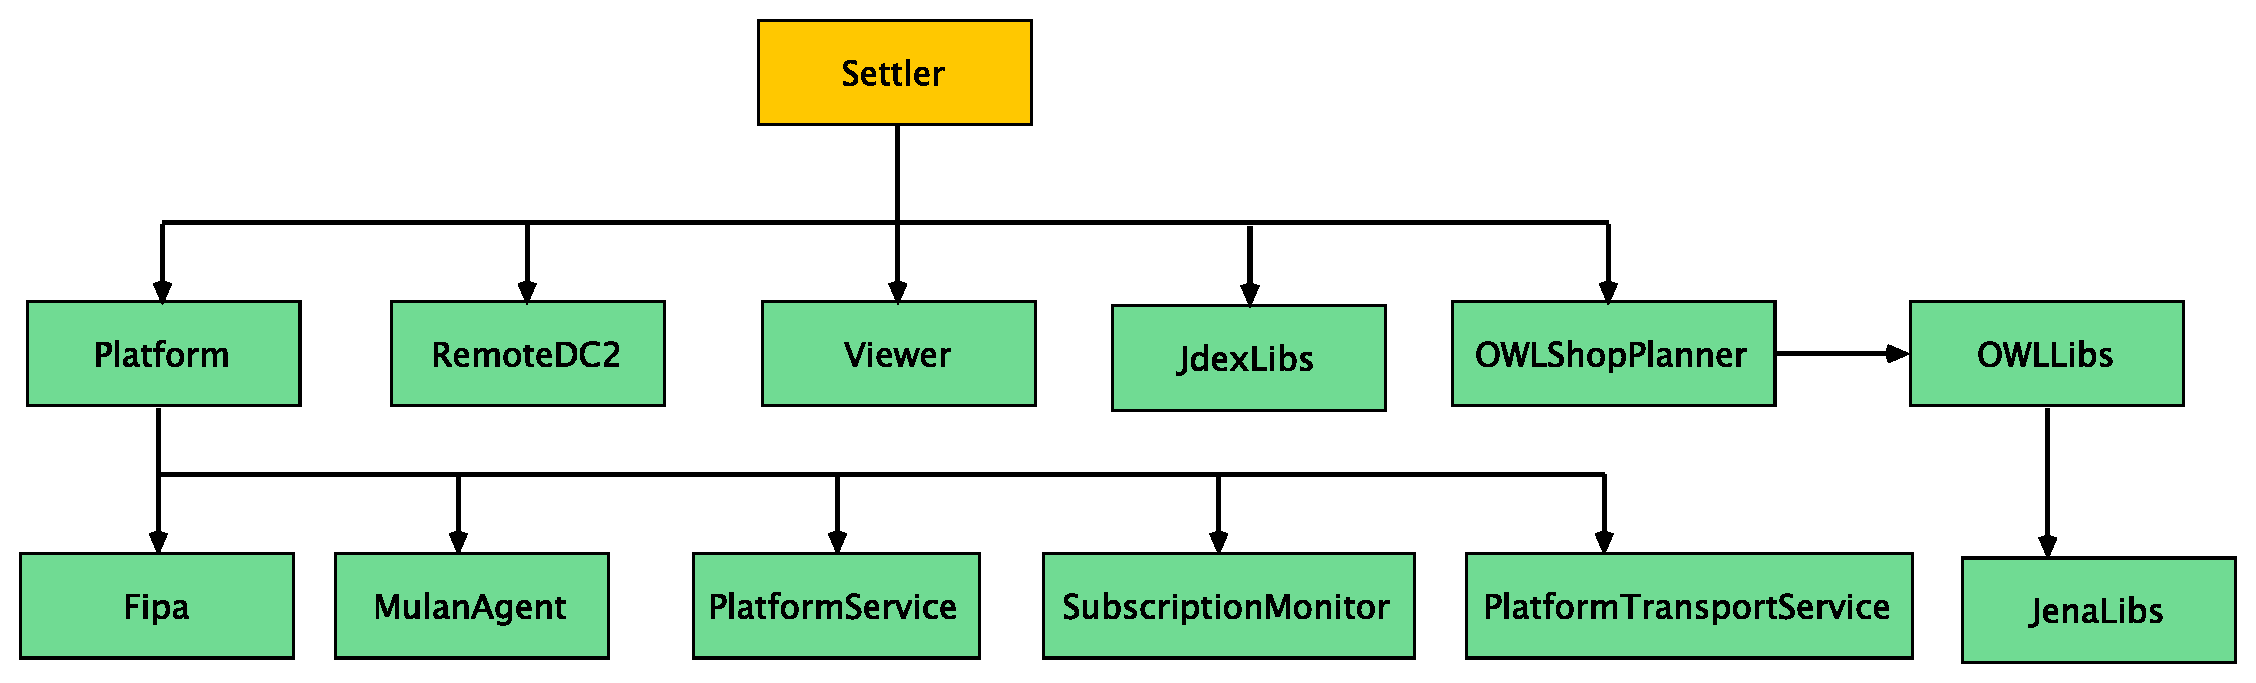
\includegraphics[width=\textwidth]{material/images/settler-mulan-plugins.pdf}
	  \caption{\textit{Settler} \textsc{Mulan} Plugin Menge}
	  \label{fig:settler_mulan_plugins}
	\end{figure}

	Im Folgenden werden die benötigten \textsc{Renew} Plugins modularisiert und zum ersten Mal das \textsc{Mulan} \textit{Settler-Target} ausgeführt. Dieses soll das \textit{Settler} Spiel mit allen nötigen Abhängigkeiten von \textsc{Mulan}, sowie \textsc{Renew} kompilieren und verpacken. Jedoch wird man während der Ausführung auf Plugin Klassen verwiesen, die für das Kompilieren notwendig sind und nicht als Teil des \textit{Settler-Targets}, sowie der \textit{plugin.cfg's}, gelistet sind. \newline
	Die Nachfolge-Analyse ergab zusätzliche Abhängigkeiten aus dem \textit{Plattform-Transport-Service}, sowie \textit{Subscription Monitor} Plugins, die ein älteres Plugin ersetzen, und noch nicht komplett in die \textit{Ant}-Umgebung eingebunden sind. Daher werden diese im \textit{Settler} \textit{Ant-Target} verankert, sowie in den \textit{CAPA} Plugin \textit{plugin.cfg} nachgerüstet. Konsequenterweise, muss der Abhängigkeitsbaum, durch die nachträglichen \textsc{Mulan}-Plugins erweitert, und auf zusätzlicher \textsc{Renew} Plugins inspiziert werden. \newline
	In den Abbildungen \ref{fig:settler_mulan_plugins} sowie \ref{fig:renew_mulan_plugins}, werden die endgültigen Plugin Mengen aus \textsc{Mulan} und \textsc{Renew} dargestellt, die \textit{Settler} für die Ausführung benötigt. \bigbreak

	\begin{figure}[h!]
	  \centering
	  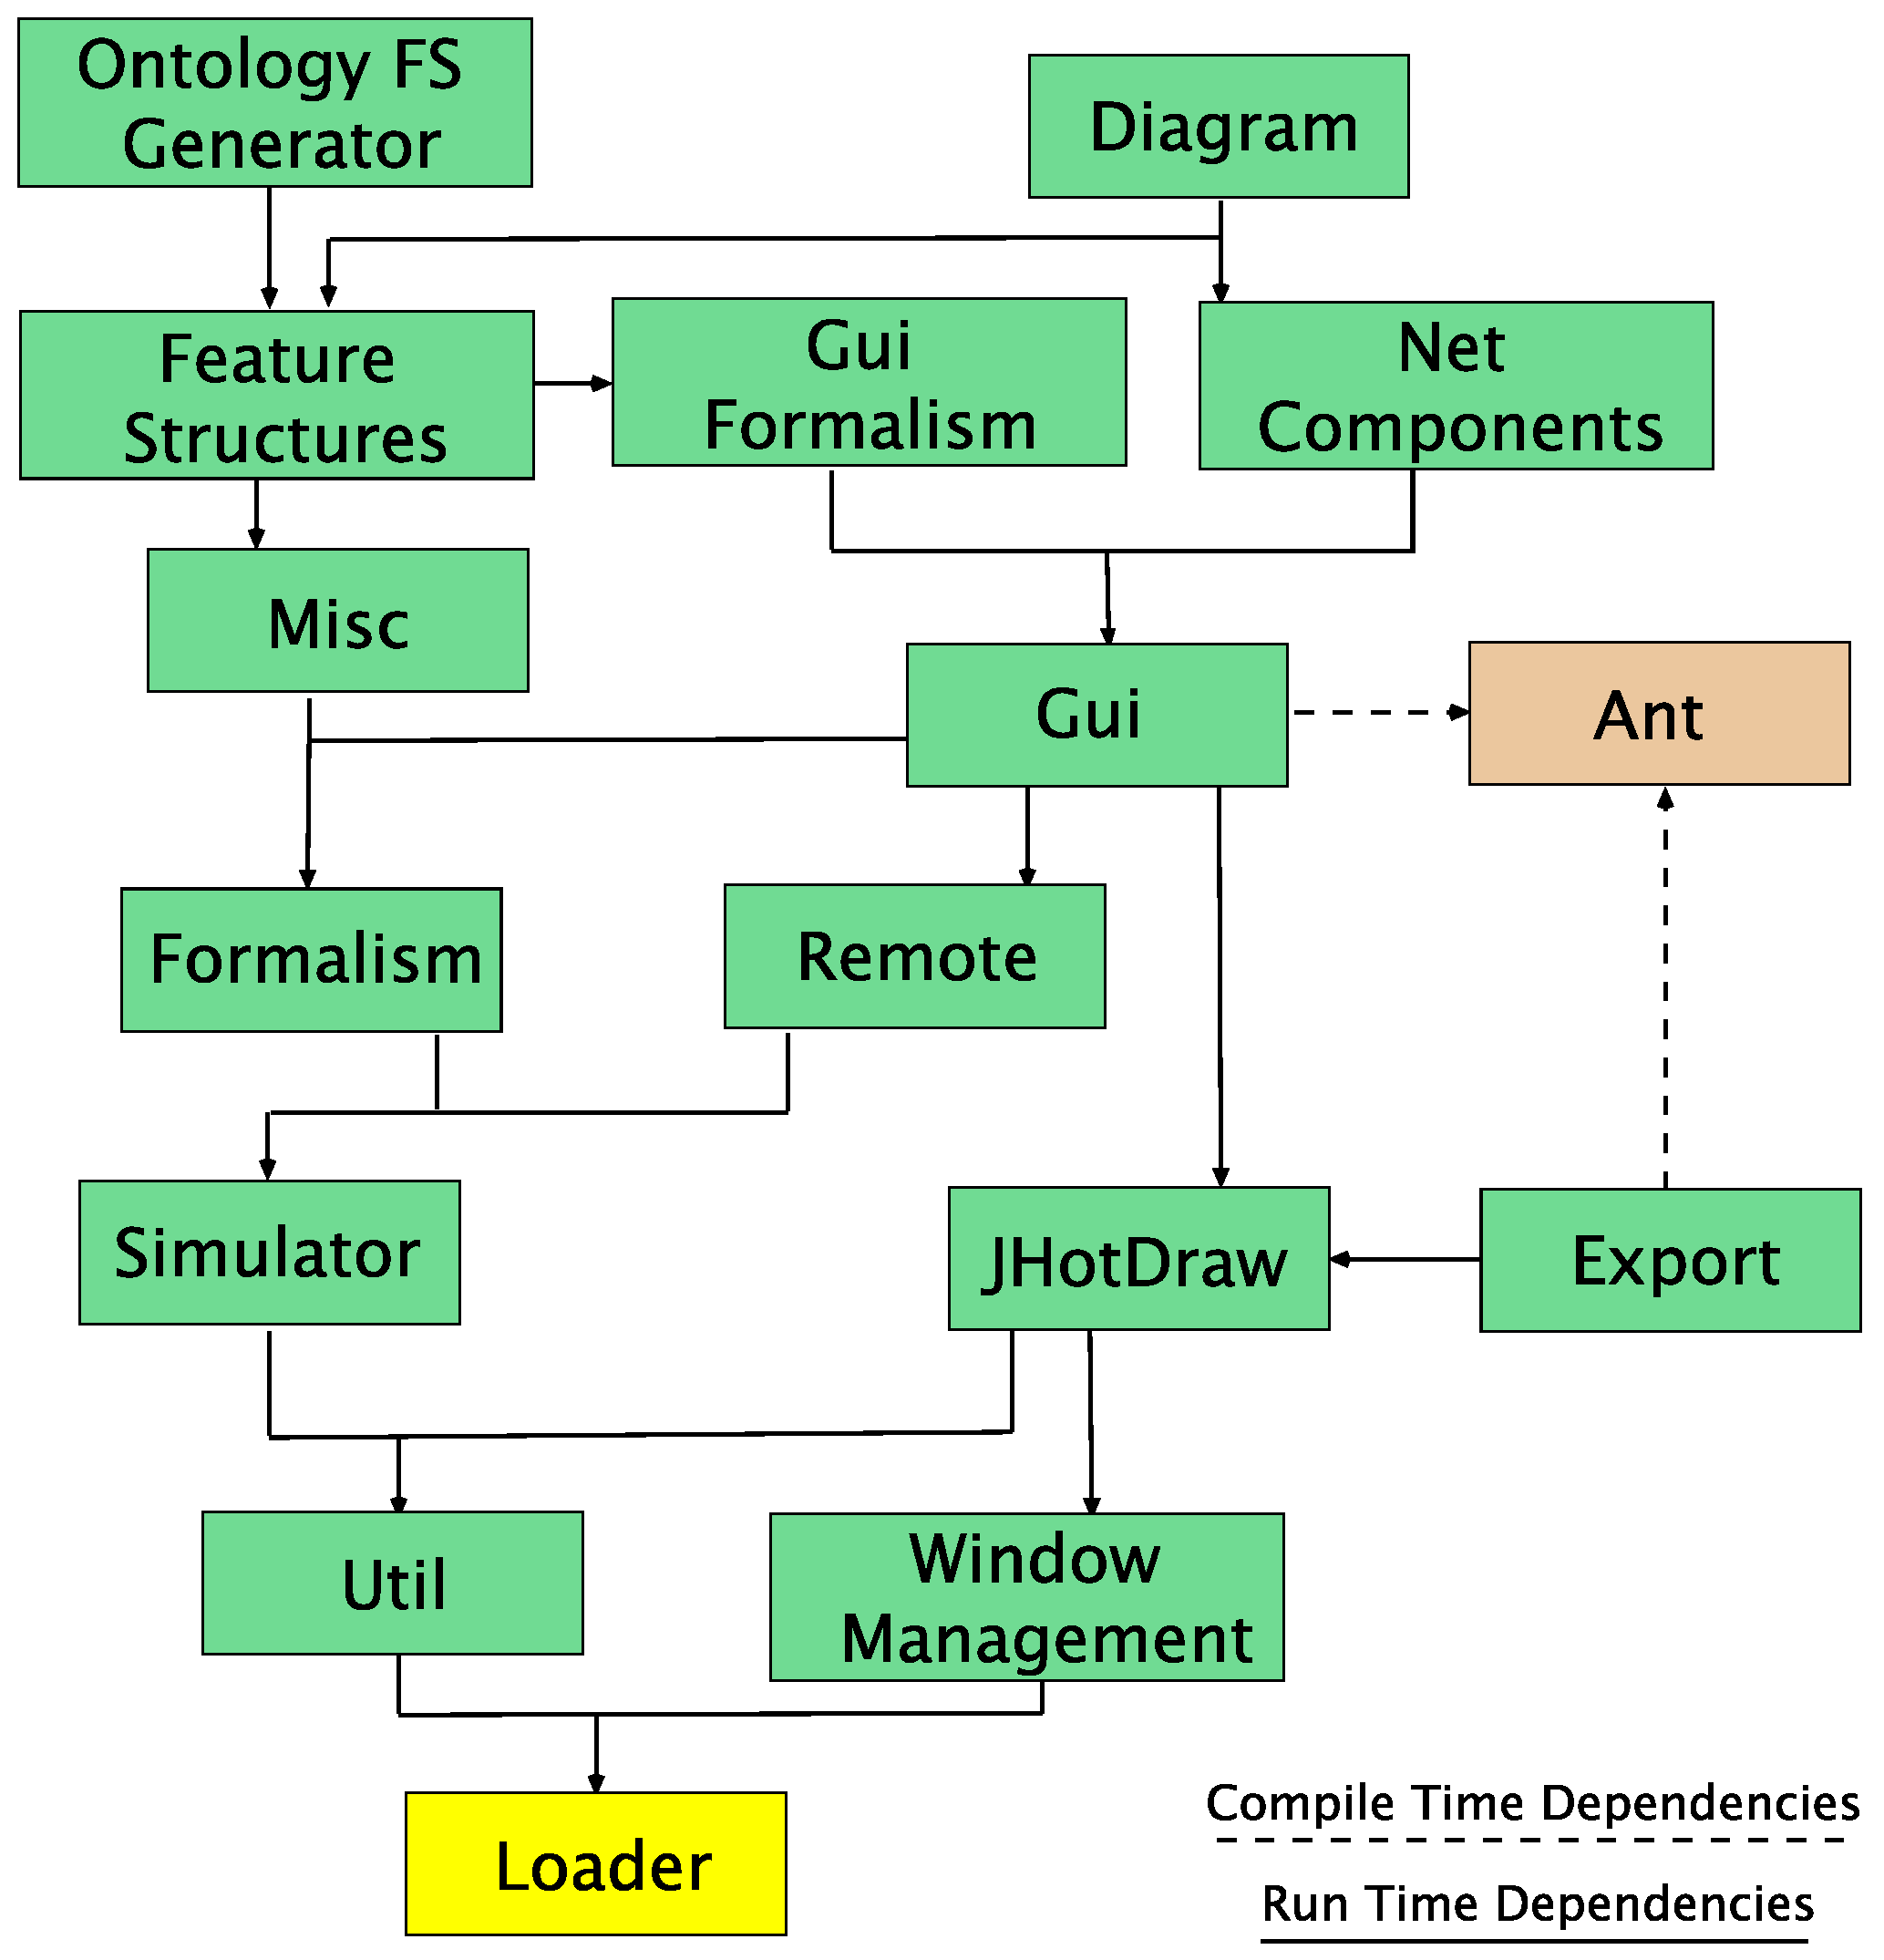
\includegraphics[width=\textwidth]{material/images/settler-renew-tree-extend.pdf}
	  \caption{Minimale modulare \textsc{Renew} Version für \textit{Settler}}
	  \label{fig:renew_mulan_plugins}
	\end{figure}	

	Im nächsten Schritt müssen die Klassenpfade innerhalb der \textsc{Mulan} Plugins angepasst werden, denn diese verweisen auf \textsc{Renew} Plugins mit der alten Projektstruktur und werden daher nicht gefunden. Um diesen Zustand zu beheben, wird die Korrektur mithilfe der regulären Ausdrücke, \textsc{Mulan} übergreifend nachgezogen und enthält letztendlich keine Referenzen auf alte und nicht existierenden Paketstrukturen von \textsc{Renew}. Die betroffenen \textsc{Mulan} Plugins sind: UseCaseComponents, YamlToFSConceptDiagram, KnowledgeRoundTrip, MulanDoc, FSOntologyGenerator, SLEditor, WF und das AgentRoleModeler Plugin. \newline
	Mit dem letzten Schritt wurden alle \textsc{Mulan} Java Klassen innerhalb der \textsc{Renew} Plugin Menge richtig verbunden. Dennoch bestehen Probleme bei der Referenzierung der Aufrufmethoden. Wie in der Einleitung angedeutet, setzt das modulare \textsc{Renew} auf \textsc{Renew} mit erweiterten Benutzeroberfläche auf und wurde bislang nur zum Teil mit \textsc{Mulan} zusammengeführt. Aus diesem Grund kann die \textit{KnowledgeBaseGenerator} Klasse aus dem AgentRoleConverter Plugin, nicht auf alle versprochenen Methoden von der erweiterten Benutzeroberfläche, zugreifen, wie zum Beispiel das Ausführen eines Speicherdialogs. Dieses Fehlverhalten wird behoben, indem \textit{Settler} auf die angepasste Schnittstelle zugreift und den entsprechenden Dialog koordiniert. \bigbreak

	\begin{figure}[h!]
	  \centering
	  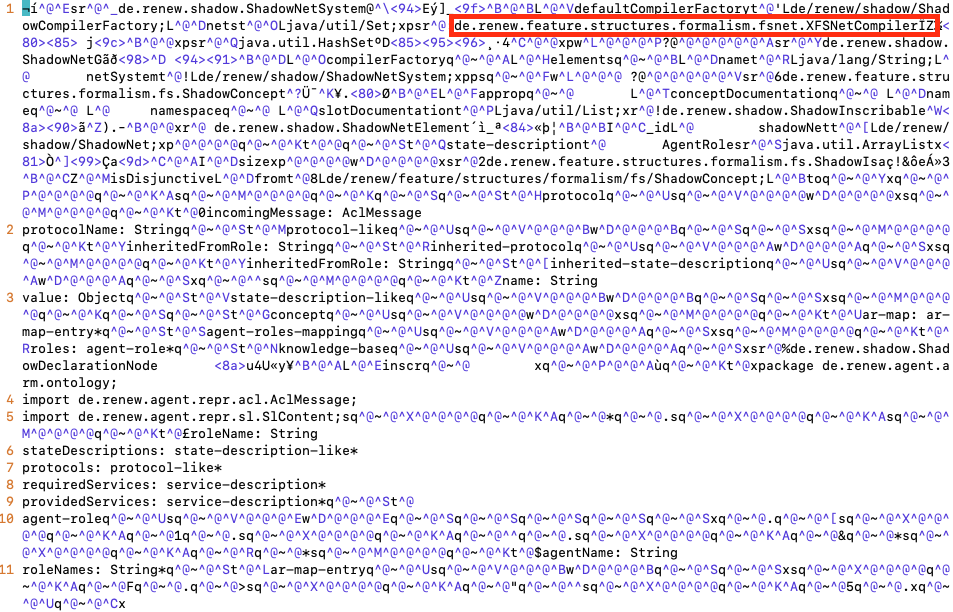
\includegraphics[width=0.8\textwidth]{material/images/shadownet.png}
	  \caption{SNS Netz}
	  \label{fig:sns_netz}
	\end{figure}

	Obwohl die Klassen, sowie Methoden miteinander verzahnt wurden, müssen jetzt zusätzlich Ressourcen, unter Verwendung des Ant Werkzeugs und speziell für \textsc{Renew} implementierte \textit{Ant-Tasks}, generiert werden. Diese nutzen Java Klassen, die in vielen Paketen der \textsc{Renew} Plugins direkt verankert sind. Somit müssen Ant Skripte für die entsprechenden \textit{Tasks} adaptiert werden. Zum Beispiel in der \textit{commonTasks.xml} für den \textit{CreateShadowNetsTask}, der sich jetzt in einem anderen Paket befindet. Dieser ist zuständig für das Kompilieren der \textsc{Renew} Zeichnungen, in ausführbare Shadow Netze. Auch wenn der \textit{CreateShadowNetsTask}, \textit{Shadow Netze} aus den \textsc{Renew} Zeichnungen generieren kann, gibt es bereits kompilierte Netze, die als einfache Ressourcen mit \textsc{Mulan} mitgeliefert werden. \newline
	Im Gegensatz zu den \textsc{Renew} Zeichnungen enthalten, die \textit{Shadow Netze} keine UI-Information, wie zum Beispiel Position oder Färbung der Netzelemente Jedoch enthalten diese Information über den genutzten Netz-Compiler, der für das Kompilieren der Datei zuständig war, und jetzt für das Öffnen zuständig sein wird. Daher müssen bereits kompilierte \textsc{Renew} Zeichnungen für die modulare \textsc{Renew}-Basis, angepasst werde. Dafür wird mithilfe eines Text-Editors und einem regulären Ausdruck, die entsprechenden Klassenverweise auf den \textit{XFSNetCompiler} aktualisiert, um dem Ausführungskontext zu entsprechen. \newline
	Das Ergebnis, sowie ein Beispiel für ein aktualisiertes \textit{Shadow Netz}, ist in der Abbildung \ref{fig:sns_netz} dargestellt. \bigbreak
	Zu diesem Zeitpunkt wurden alle Mängel und Uneindeutigkeiten zwischen \textit{Settler}, \textsc{Mulan} und den modularen \textsc{Renew} beseitigt, dennoch fehlt für die Ausführung der \textdc{Mulan}-\textit{Settler} Variation,  die Zeichnung \textit{settler.rnw}. Dieses befindet sich im \textit{Settler}-Plugin-Projekt und wird nicht in der Standardausführung mitgeliefert, sondern bei Bedarf mit einem \textit{sh} Skript während des Starts nachgeladen. \newline
	Da die Umsetzung der \textdc{Mulan}-\textit{Settler} Variation auf das \textit{Settler} Spiel abzielt, wird dieses Skript im \textit{Ant-Build} Prozess verankert und in das \textit{Settler}-Plugin mitkompiliert und verpackt. \newline

	\begin{figure}[h!]
	  \centering
	  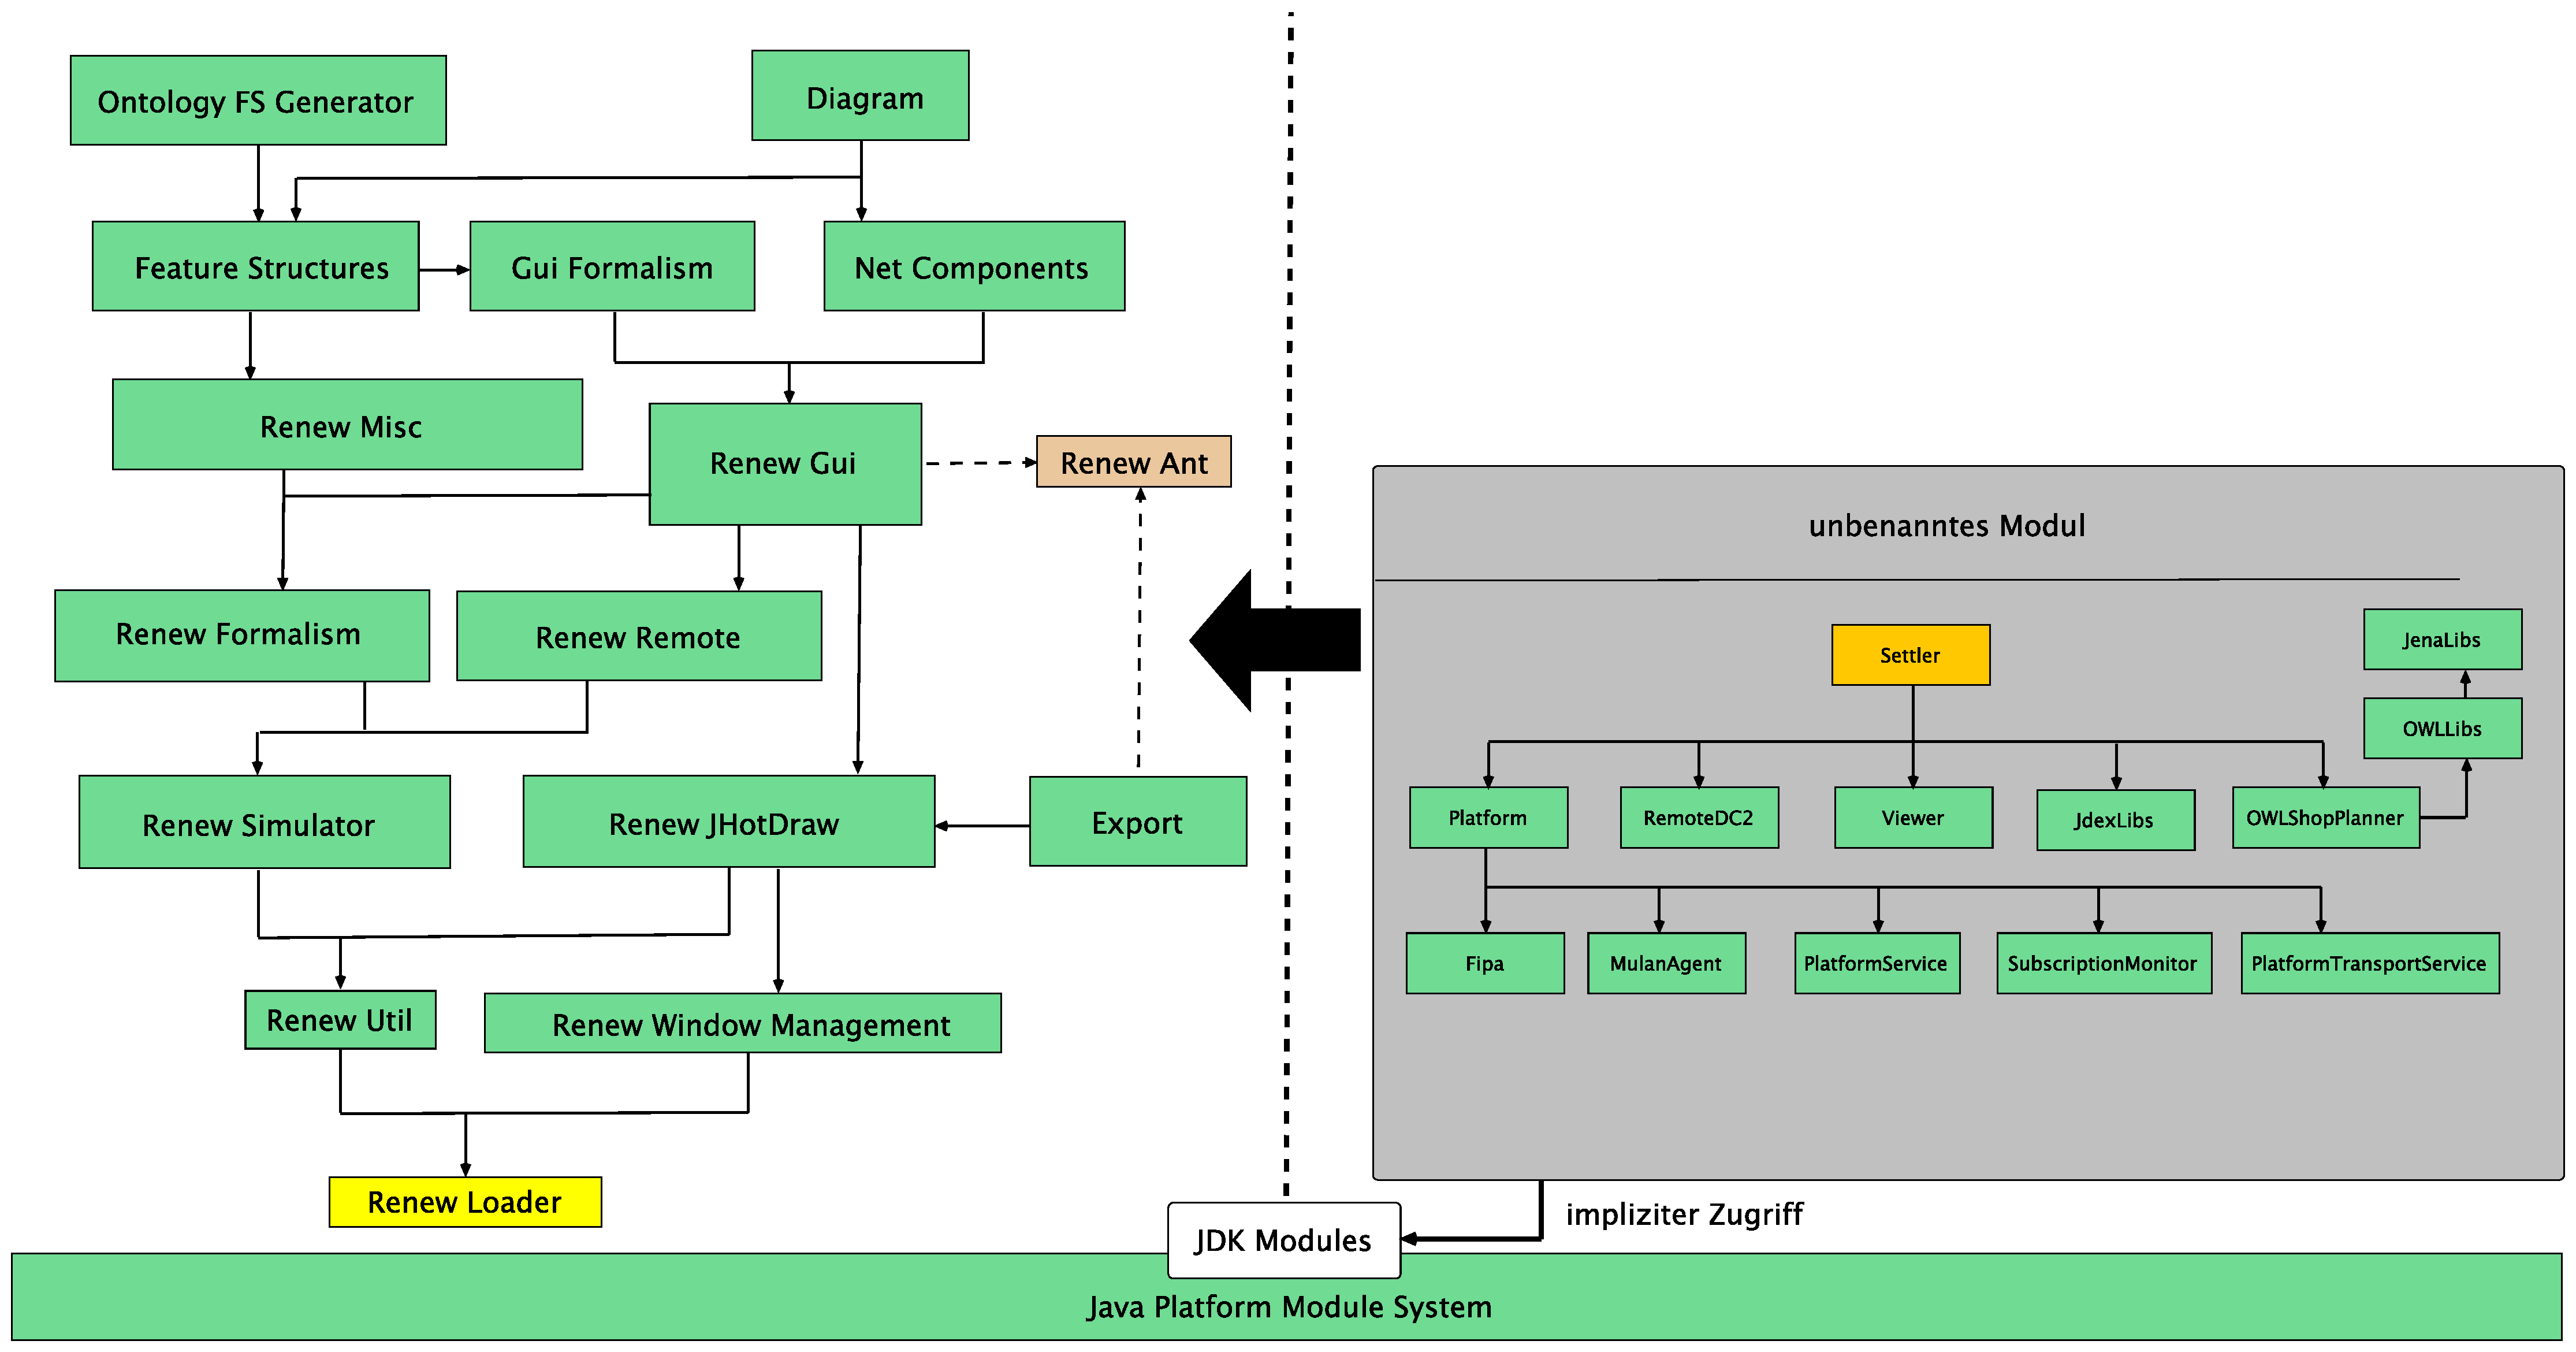
\includegraphics[width=\textwidth]{material/images/settler-renew-mulan-vm.pdf}
	  \caption{\textit{Settler}-\textsc{Mulan} Variation}
	  \label{fig:mul_prot}
	\end{figure}

	Jetzt ist das \textit{Settler} Spiel für die Ausführung bereit, und enthält alle nötigen Konfigurationen für das modulare \textsc{Renew}, mit der erweiterten Oberfläche. Dafür wurden zahlreiche Anpassungen durchgeführt, die eine Brücke zwischen der \textsc{Mulan}-\textit{Settler} Variation und dem modularen \textsc{Renew}, bilden. Es wurden Plugins modularisiert, Ressourcen angepasst, Skripte umgeschrieben und kleine Mängel behoben. \newline
	In der Abbildung \ref{fig:mul_prot} ist der fertige Prototyp abgebildet, der die Spezifikation erfüllt und als ein praktisches Beispiel für die Migration einer existierenden Software dient. 

\section{Evaluation}
	Der entstandene Prototyp deckt ein Migrationsszenario ab, das innerhalb eines Projektes mit einer großen Codebasis, entstehen könnte. Die Erwartung eines nahtlosen Austausches von \textsc{Renew} gegen das modulare \textsc{Renew}, hat sich nicht ergeben. Alle Änderungen, die in den entstehenden Prototypen resultieren, erfordern für das initiale Aufsetzen von existierendem Alt-Code auf modulare Grundlagen, einen mittleren Aufwand. Es müssen Pfade, Ressourcen und Prozesse angepasst werden, die voraussichtlich alle Bereiche einer Applikation betreffen werden.\newline
	Dennoch ergaben sich auch positive Resultate, denn das Erweitern der existierenden Modulmenge, ergab ein einfaches, übersichtliches und nachhaltiges Verfahren, welches sich in der erweiterten \textsc{Renew}--Minimalkonfiguration, erwiesen hat. Mit jedem weiteren modularisierten Plugin, wurde das Hinzufügen von Plugins zu der Gesamtumsetzung , immer simpler und verlangte keinen nennenswerten Aufwand für die benötigen Abhängigkeiten. Zusätzlich steigt ab einem gewissen Punkt die Unterstützung für das Koppeln der Module mit einer intelligenten \textit{IDE}, und bildet somit ein neues, willkommenes Hilfsmittel.
